\documentclass[12pt,twoside,bind,ams,a4paper]{hepthesis}
\usepackage[utf8]{inputenc}
\usepackage[T1]{fontenc}
\usepackage[ngerman]{babel}
\usepackage{lmodern,hfoldsty,charter}
% Schriftarten: Variante 2
%\usepackage{charter}
% Paket fuer mathematische Symbole
\usepackage{amssymb}
% Paket fuer Literaturverzeichnis nach DIN
%\usepackage{natbib}
% Literaturzitate in eckige Klammern setzen
%\setcitestyle{square}

% Paket zum Einbinden von ein- oder mehrseitigen PDFs
\usepackage{pdfpages}
\usepackage{url}
% Paket zur typographisch richtigen Angabe von Groessen mit SI-Masseinheiten
\usepackage[squaren]{SIunits}
% Paket fuer Bra-/Ket-Vektor-Schreibweise, mit automatischer Groessenanpassung
\usepackage{braket}

\title{Impact of stellar variability on the observational appearance of protoplanetary disks}
\author{Alexandra Botnariuc}

\begin{document}

\begin{frontmatter}
%titel page
\thispagestyle{empty}
\begin{center}
\vspace*{-2cm}

\includegraphics[width=0.75\textwidth]{unilogo-siegel-farbe}\\
\vspace*{3cm}
    {\titlefont \huge \onehalfspacing
	\thetitle 
    \par}
   \vfill
	\Large{\uppercase{Master Thesis}} 

\end{center}\par

\vspace{1cm}

\begin{center}
\textbf{
	in fulfillment of the requirements for the Degree of \\
	\vspace{5mm}
	{\Large Master of Science} \\
	\vspace{5mm}
	in Computational Science and Engineering with Physics \\
	submitted to the Faculty of Computer Science and Electrical Engineering, \\
	University of Rostock}
\end{center}
\vspace*{1cm}
\noindent\begin{minipage}[b]{\textwidth}
{
\noindent Author: Alexandra Botnariuc \\
\vspace*{1.5cm}

	\begin{tabbing}
	Advisor:  \= Prof. Dr. S. Wolf, CAU Kiel\\
	Co-advisor: \=  Prof. Dr. R. Redmer, Universität Rostock \\
	\end{tabbing}

  \noindent Rostock, 11 January 2019
  \par
  }
\end{minipage}




\begin{abstract}[Abstract]
\thispagestyle{plain}
Summary here!
\end{abstract}

\tableofcontents

\end{frontmatter}

\begin{mainmatter}
\chapter{Einleitung}
\label{kap-einleitung}

% Seitennummerierung auf arabische Zahlen umstellen, neu beginnend im Kapitel 1
\pagenumbering{arabic}

\chapterquote{Ach, die Physik! Die ist ja für die Physiker viel zu schwer!}{David Hilbert (Bsp. für Einbindung eines einleitenden Zitats)}

Der Umfang der Bachelorarbeit sollte 20-30 Seiten betragen, der Umfang einer Masterarbeit 40-80 Seiten.
Dabei sind das Deckblatt, das  Inhaltsverzeichnis  und  die  Angaben  zur  verwendeten  Literatur  nicht  zu  zählen, sondern nur die reinen Textseiten, einschließlich der Abbildungen.

Die Gliederung und der Inhalt der Kapitel sind mit dem Betreuer der Arbeit abzusprechen. Maßgebend für inhaltliche und formale Anforderungen sind natürlich die (Bachelor, Master)-\-Prüfungs\-ordnungen.

\paragraph{Technische Hinweise:}
\begin{itemize}
  \item Grundlayout und Strukturierung dieser Vorlage basieren auf der Latex-Klasse ``hepthesis'' von Andy Buckley. Im Ordner ``anleitungen'' findet sich die Anleitung mit weiteren Optionen und Befehlen hierzu.
  \item Die Literaturliste orientiert sich an der DIN 1505. Dazu werden das Paket ``natbib'' mit erweiterten Zitationsbefehlen (s.a. Ordner ``anleitungen'') und die Stile (*.bst-Dateien) aus dem ``din1505''-Paket verwendet. 
  \item Das Dokument ist mit ``pdflatex'' zu übersetzen, also \textit{pdflatex abschlussarbeit} auf der Kommandozeile bzw. im Latex-Editor ``Kile'' mit der Projekt-Einstellung ``Schnell\-erstellung: PDF-Latex + ViewPDF''.
  \item Die Literaturliste im Dokument wird mit Hilfe der Literaturdatenbank (*.bib-Datei) erzeugt. ``Kile'' erledigt das automatisch. Der entsprechende Kommando\-zeilen-Befehl lautet \textit{bibtex abschlussarbeit}, danach muss noch einmal \textit{pdflatex abschlussarbeit} folgen. Dieser Vorgang muss -- wie bei Latex üblich -- eventuell mehrfach wiederholt werden.
  \item Umlaute und Sonderzeichen: Man muss darauf achten, dass die in der Latex-Präambel angegebene Code-Tabelle (\textit{usepackage inputenc}-Befehl) mit der im Latex-Editor verwendeten übereinstimmt. Neuere Linux-Distributionen verwenden automatisch Unicode (UTF8), damit werden im Prinzip alle bekannten Sonderzeichen und selbst nicht-lateinische Schriften wie kyrillisch, wie getippt angezeigt.
\end{itemize}

Hier folgt der Text zu Kapitel 1 mit Literaturverweisen wie \cite{Jackson1999,Einstein1925} oder
\cite{HaugKoch2004,Meinke2005,Holm1998}.

\section{Physikalische Grundlagen}
Der Hamiltonoperator eines Teilchens ist \cite{Nolting2007}
\begin{equation}\label{ham}
\hat{H}=\frac{\hat{\vec{p}\,}^2}{2m}\,+\,V(\hat{\vec{r}}\,)
\end{equation}
Der Erwartungswert der Energie ergibt sich aus 
\begin{align}
  \label{gl-erwartungswert}
  \Braket{\Psi_0|\hat H|\Psi_0} = E,
\end{align}
mit dem Hamiltonoperator aus Gl.\ \eqref{ham}.


\section{Besonderheiten des verwendeten Materials}

\subsection{Effektive-Massen-Näherung}
weitere Untergliederung m\"oglich

\chapter{Theorie}
\label{kap-theorie}

Nach den einleitenden Bemerkungen in Kapitel \ref{kap-einleitung} mit der fundamentalen Gleichung 
 \eqref{gl-erwartungswert} geht es jetzt weiter. Die Definition des Kreises ist illustriert 
in Abb.~\ref{fig-kreis}.

\begin{figure}
% Rather than specifying figure widths in raw terms, like centimetres, or docu-
% ment parameters like \textwidth, it’s nice to be able to have a more semantic
% reference. Having a few standard width also helps to keep things looking con-
% sistent through the document. For these reasons, hepthesis provides four
% standard figure widths, \smallfigwidth, \mediumfigwidth, \largefigwidth
% and \hugefigwidth, which are defined in terms of the text width and chosen
% to avoid overflows. Use them like this:
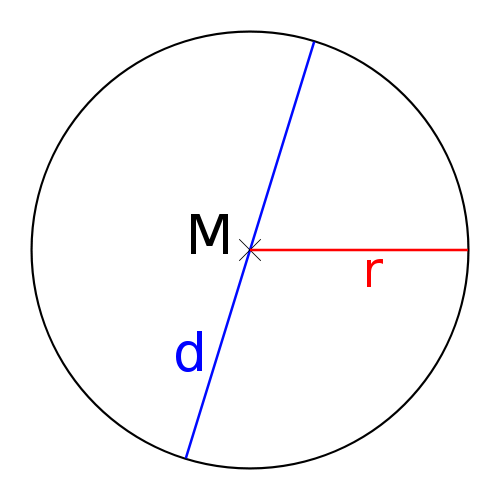
\includegraphics[width=\mediumfigwidth]{img/kreis.png}
\caption{Ein Kreis ist die Menge aller Punkte, die von einem gemeinsamen Mittelpunkt den gleichen Abstand haben.  Hier wird eine PNG-Grafik eingelesen.}
\label{fig-kreis}
\end{figure} 

\pagebreak
\section{Hamilton-Operator des Systems}
In  Abb.~\ref{fig-quadrat} wird das Quadrat gezeigt.

\begin{figure}[h]
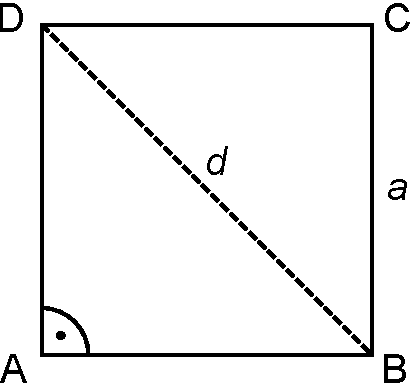
\includegraphics[width=\smallfigwidth]{img/quadrat.pdf}
\caption{Ein Quadrat ist etwas völlig anderes als ein Kreis (siehe Abb.\ \ref{fig-kreis}). 
Hier wird ein PDF-File als Grafik eingelesen.}
\label{fig-quadrat}
\end{figure} 



\section{Störungstheoretische Betrachtung}

\end{mainmatter}

% Anhaenge -- auskommentieren falls nicht ben\"{o}tigt.
\begin{appendices}
\chapter{Zahlen}
Ein Beispiel f\"ur eine Tabelle: Die Zahlen sind gegeben in Tabelle \ref{tab-zahlen}.

\begin{table}
\begin{center}
\begin{tabular}{c|c}
Nr. & Zahl \\
\hline{} \\
1 & 1\\
2 & 2\\
3 & 3\\
4 & 4\\
5 & 5\\
6 & 6\\
7 & 7\\
8 & 8\\
9 & 9\\
10 & 10 \\
\end{tabular}
\end{center}
\caption{Die Zahlen von 1 bis 10. Zitiert nach \cite{HaugKoch2004}.}
\label{tab-zahlen}
% Beachte: Das Label muss immer nach der Caption kommen!
\end{table} 

\end{appendices}

\begin{backmatter}
% Verweis auf Literaturverzeichnis zum Inhaltsverzeichnis hinzufuegen
\addtocontents{toc}{\vspace*{1em}}

% Literaturliste aus Literaturdatenbank (Bibtex-Datei) bauen. Nur tatsaechlich zitierte Literatur wird in Liste aufgenommen.
% Regelmaessigen Aufruf von ``bibtex abschlussarbeit'' nicht vergessen, falls das der Latex-Editor nicht
% erledigt.
% Zur Bearbeitung der Literaturdatenbank kann das Programm JabRef (http://jabref.sf.net) empfohlen werden. (Java-Programm, laeuft unter Windows, Linux, Mac, ...)
\bibliography{literatur}
% Stil fuer Literaturliste festlegen
% Variante A: DIN, Eintraege erhalten Kuerzel aus Autoren-Initialien und Jahr, alphabetisch geordnet
%\bibliographystyle{alphadin}
% Variante B: DIN, Eintraege werden durchnummeriert, alphabetisch geordnet
\bibliographystyle{abbrvdin}


\begin{abstract}[Selbstständigkeitserklärung]
\thispagestyle{empty}
Ich versichere hiermit, dass ich die vorliegende Arbeit selbstständig
verfasst und keine anderen als die angegebenen Quellen und Hilfsmittel benutzt habe.
\vspace*{2cm}

\flushright{
Rostock, (Datum)
}
\end{abstract}

\end{backmatter}

\end{document}
